
%(BEGIN_QUESTION)
% Copyright 2015, Tony R. Kuphaldt, released under the Creative Commons Attribution License (v 1.0)
% This means you may do almost anything with this work of mine, so long as you give me proper credit

According to Rosemount recommendations, a {\sl Wireless}HART instrument's antenna should be vertically oriented, and given plenty of space between it and any ``objects in a parallel metal plane such as a pipe or a metal framework.''  Explain why there is a concern over metal objects lying {\it parallel} to the antenna, more so than metal objects {\it perpendicular} to the antenna.

\vskip 10pt

Also, identify the major problem with this {\sl Wireless}HART transmitter installation and suggest improvements for it:

$$\includegraphics[width=15.5cm]{i04602x01.eps}$$

\vskip 20pt \vbox{\hrule \hbox{\strut \vrule{} {\bf Suggestions for Socratic discussion} \vrule} \hrule}

\begin{itemize}
\item{} Which information in this illustration is relevent to the question, and which is not?
\item{} Suggest alterations in this system to improve the performance of the {\sl Wireless}HART network.
\end{itemize}

\underbar{file i04602}
%(END_QUESTION)





%(BEGIN_ANSWER)


%(END_ANSWER)





%(BEGIN_NOTES)

The {\sl Wireless}HART devices are located much too closely to the (conductive) concrete slab floor.  They need to be elevated more!  The {\sl Wireless}HART System Engineering Guide (revision 2.2) cites 2 meters as a minimum criterion (in addition to an obstructionless path) in order to achieve the advertised communication range of 750 feet (page 38 of 82).

\vskip 10pt

A particular challenge in this system is the flow transmitter, which must be mounted underneath the pipe (i.e. close to the floor) because its impulse lines must be filled with process liquid.  One possible solution is to use a regular wired-HART device for this flow transmitter, then wire a THUM (located at some high elevation) for better radio reception.

%INDEX% Electronics review: antenna mounting orientation
%INDEX% Electronics review: antenna type
%INDEX% Networking, WirelessHART

%(END_NOTES)


